\documentclass{ximera}

\title{Triangular numbers}

\newcommand{\defnword}[1]{\textbf{#1}}
\newcommand{\ds}{\displaystyle}
\newcommand{\Z}{\mathbb{Z}}
\newcommand{\N}{\mathbb{N}}
\newcommand{\nth}{\mbox{\scriptsize th}}
\renewcommand{\index}[1]{}

\begin{document}

\begin{abstract}
  The triangular numbers are an example of a sequence.
\end{abstract}

\maketitle

\subsection{Triangular numbers}

The sequence of \defnword{triangular numbers} $(T_n)$ is a sequence of
integers counting the number of dots in increasingly large
``equilateral triangles'' built from dots.  The term $T_n$ is the
number of dots in a triangle with $n$ dots to a side.

\begin{fullwidth}
\begin{figure*}[!h]
\begin{minipage}{0.6in}
\begin{center}

\begin{tikzpicture}[y=0.5cm,x=0.3415cm]
\fill (0,0) circle (3pt);
\end{tikzpicture} \\
$T_1 = 1$
\end{center}
\end{minipage}
\begin{minipage}{1.1in}
\begin{center}

\begin{tikzpicture}[y=0.5cm,x=0.3415cm]
\fill (0,0) circle (3pt);
\fill (1,-1) circle (3pt);
\fill (-1,-1) circle (3pt);
\end{tikzpicture} \\
$T_2 = 3$
\end{center}
\end{minipage}
\begin{minipage}{1.2in}
\begin{center}
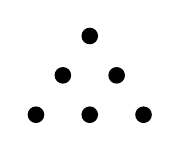
\begin{tikzpicture}[y=0.5cm,x=0.3415cm]
\fill (0,0) circle (3pt);
\fill (1,-1) circle (3pt);
\fill (-1,-1) circle (3pt);
\fill (-2,-2) circle (3pt);
\fill (0,-2) circle (3pt);
\fill (2,-2) circle (3pt);
\end{tikzpicture} \\
$T_3 = 6$
\end{center}
\end{minipage}
\begin{minipage}{1.3in}
\begin{center}
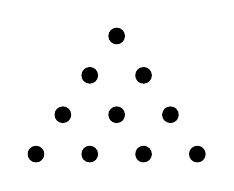
\begin{tikzpicture}[y=0.5cm,x=0.3415cm]
\fill (0,0) circle (3pt);
\fill (1,-1) circle (3pt);
\fill (-1,-1) circle (3pt);
\fill (-2,-2) circle (3pt);
\fill (0,-2) circle (3pt);
\fill (2,-2) circle (3pt);
\fill (-3,-3) circle (3pt);
\fill (-1,-3) circle (3pt);
\fill (1,-3) circle (3pt);
\fill (3,-3) circle (3pt);
\end{tikzpicture} \\
$T_4 = 10$
\end{center}
\end{minipage}
\begin{minipage}{1.5in}
\begin{center}
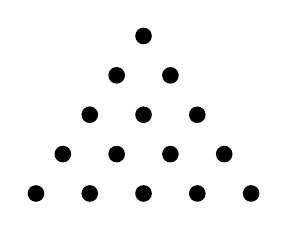
\begin{tikzpicture}[y=0.5cm,x=0.3415cm]
\fill (0,0) circle (3pt);
\fill (1,-1) circle (3pt);
\fill (-1,-1) circle (3pt);
\fill (-2,-2) circle (3pt);
\fill (0,-2) circle (3pt);
\fill (2,-2) circle (3pt);
\fill (-3,-3) circle (3pt);
\fill (-1,-3) circle (3pt);
\fill (1,-3) circle (3pt);
\fill (3,-3) circle (3pt);
\fill (-4,-4) circle (3pt);
\fill (-2,-4) circle (3pt);
\fill (0,-4) circle (3pt);
\fill (2,-4) circle (3pt);
\fill (4,-4) circle (3pt);
\end{tikzpicture} \\
$T_5 = 15$ \\
\end{center}
\end{minipage}
\begin{minipage}{1.7in}
\begin{center}
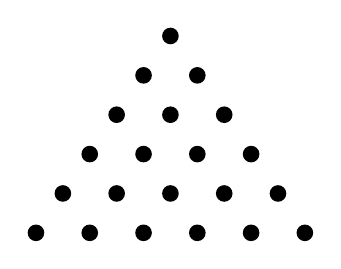
\begin{tikzpicture}[y=0.5cm,x=0.3415cm]
\fill (0,0) circle (3pt);
\fill (1,-1) circle (3pt);
\fill (-1,-1) circle (3pt);
\fill (-2,-2) circle (3pt);
\fill (0,-2) circle (3pt);
\fill (2,-2) circle (3pt);
\fill (-3,-3) circle (3pt);
\fill (-1,-3) circle (3pt);
\fill (1,-3) circle (3pt);
\fill (3,-3) circle (3pt);
\fill (-4,-4) circle (3pt);
\fill (-2,-4) circle (3pt);
\fill (0,-4) circle (3pt);
\fill (2,-4) circle (3pt);
\fill (4,-4) circle (3pt);
\fill (-5,-5) circle (3pt);
\fill (-3,-5) circle (3pt);
\fill (-1,-5) circle (3pt);
\fill (1,-5) circle (3pt);
\fill (3,-5) circle (3pt);
\fill (5,-5) circle (3pt);
\end{tikzpicture} \\
$T_6 = 21$ \\
\end{center}
\end{minipage}
\vspace{12pt}

\caption{The first six triangular numbers}
\end{figure*}
\end{fullwidth}

There are a couple of ways of making this discussion more precise.
Given an equilateral triangle with $n$ dots to a side, how many more
dots do you need to build the equilateral triangle with $n+1$ dots to
a side?  All you need to do to transform the smaller triangle to the
larger triangle is an additional row of $n+1$ dots placed along any
side.  Therefore,
\[
T_{n+1} = T_n + (n+1).
\]
Since $T_1 = 1$, this recursive definition suffices to determine the
whole sequence.

But there are other ways of computing $T_n$.  Indeed, you may recall
the explicit formula
$$
T_n = \frac{n \cdot (n+1)}{2}
$$
from Calculus One.

\end{document}
